El plan de pruebas corresponde a las descritas en [\ref{sec:BancoDePruebas}].
Para el uso correcto de los módulos se tuvieron en cuenta los siguientes aspectos:
\begin{itemize}
	\item Definir un estado predeterminado del Bus $I^2C$ mediante \textit{pullups}.
	\item El uso de capacitores de desacople
	\item Para el módulo RTC, el integrado DS1307 requiere $5 \ V$ para funcionar correctamente, por lo que para que sea compatible con la lógica de $3.3 \ V$ de la \rspi, se realiza un cambio en el esquemático al remover dos resistores del módulo.
\end{itemize}

\begin{figure}[H]
	\centering
	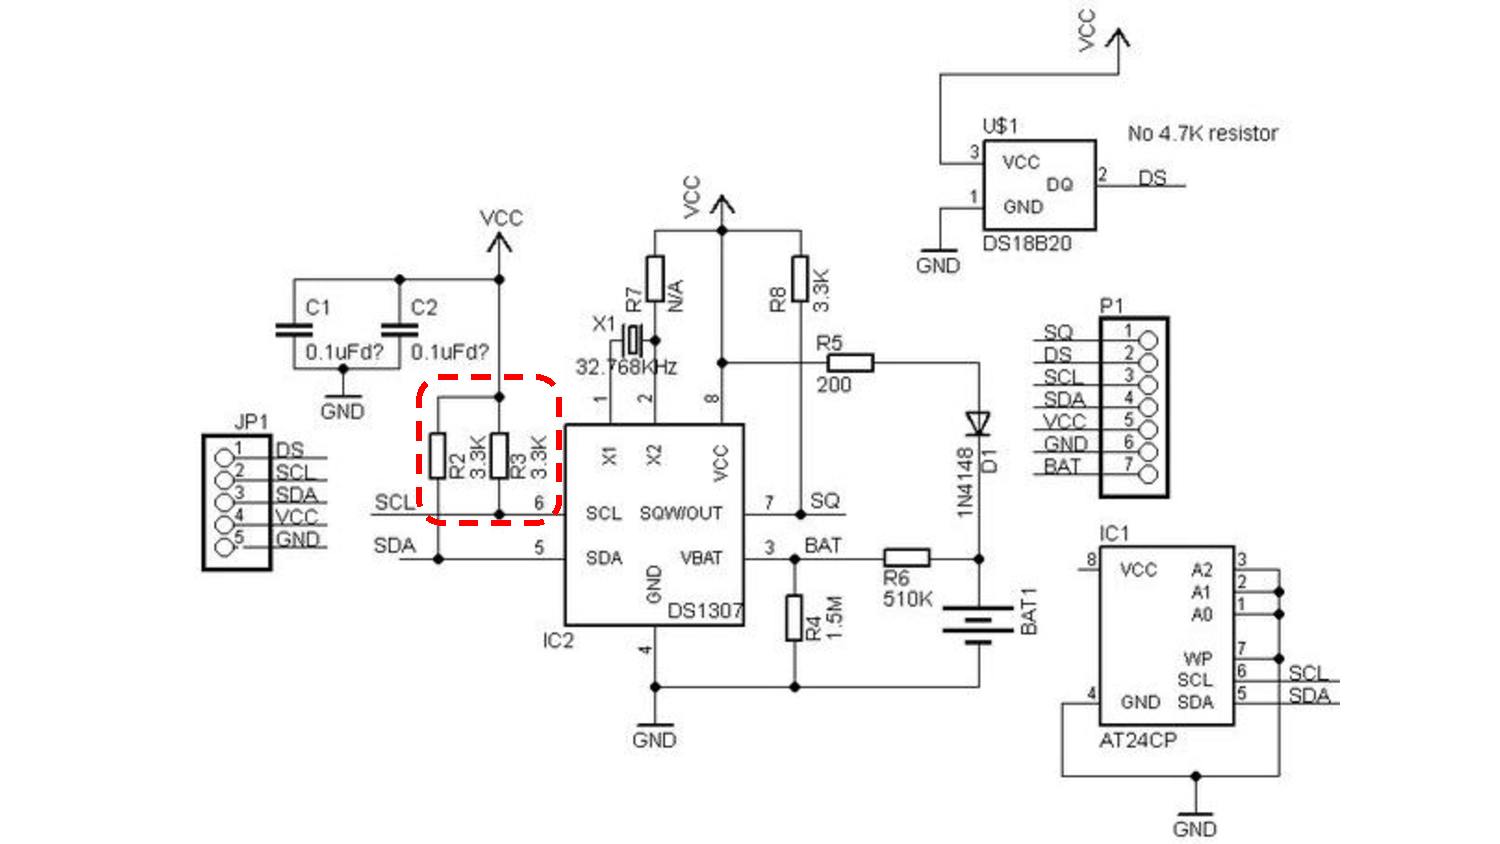
\includegraphics[width=0.9\linewidth,page=1]{ImagenesIngenieria de detalle/rtcTinySchematic}
	\caption{Esquemático RTC-Tiny.}
	\label{fig:RTCSchematic}
\end{figure}

Con este cambio se quita la referencia a $5 \ V$ del bus en el módulo. Por lo que la lógica queda en el rango de $3.3 \ V$ a $5 \ V$. Cabe destacar que utilizar los niveles lógicos de $3.3 \ V$ son compatibles con el integrado $DS1307$


